\section{Numerical work}

We wish to confirm the numerical results from
\textcite{prl-selffocus}, that is we wish to show, that a gaussian
beam is focused when propagating in a Kerr lense.

The partial differential equation given in Eqn.~\eqref{eq:kerr-diff} is categorized as a 1D
diffusion problem. A method to solve this problem is the Crank-Nicolson method which applies for
equations of the form
\begin{equation}
  \label{eq:Crank-Nicolson}
  \pdiff{u}{t} = F \Big(u, x, t, \pdiff{u}{x}, \ppdiff{u}{x} \Big), 
\end{equation}
which is also the case for our equation, since it can be rewritten as
\begin{equation}
  \label{eq:kerr-diff-crank}
  i\pdiff{E}{z} = -\half \left[\frac{1}{r} \pdiff{E}{r} + \ppdiff{E}{r} + |E|^{2} E \right]. 
\end{equation}

In order to evaluate this numerically we discretize $z$ and $r$ in order to make a grid. The first
and second order derivatives can then be approximated by the central finite difference
\begin{equation}
  \label{eq:central-diff}
  f'(x) = \frac{f(x+\half h) - f(x - \half x)}{h} \quad f''(x) = \frac{f(x+h) - 2f(x) + f(x-h)}{h^{2}}.
\end{equation}

The Crank-Nicolson method then relates the value of $E$ at the $n+1$ $z$-step to the value in the
$n$'th step via the equalities of the forward and backward euler method. Note that $i$ denote the
step in $r$
\begin{equation}
  \label{eq:Crank-Nicolson-discrete}
  \frac{E^{n+1}_{i} - E^{n}_{i}}{\Delta z} = \half \big[F_{i}^{n+1}+F_{i}^{n} \big].
\end{equation}
The right hand side of the can be evaluated using the central difference approximation. This gives
a set of equations for $E^{n+1}$ that depends on $E^{n}$ ie. the values in the previous step
\begin{align}
  \notag
  (\alpha + 2\beta^{2} - |E_{i}^{n+1}|^{2})E_{i}^{n+1} - \beta^{2}(E_{i+2}^{n+1} + E_{i-2}^{n+1}) -
  \frac{\beta}{r_{i}} (E_{i+1}^{n+1} - E_{i-1}^{n+1}) \\
  = (\alpha - 2\beta^{2} + |E_{i}^{n}|^{2})E_{i}^{n} + \beta^{2}(E_{i+2}^{n} + E_{i-2}^{n}) +
  \frac{\beta}{r_{i}} (E_{i+1}^{n} - E_{i-1}^{n}), 
  \label{eq:kerr-long}
\end{align}
where $\alpha = -2i/\!{\Delta z}$ and $\beta = 1/{2 \Delta r}$.

This is almost a fivediagonal matrix equation except for the term that is cubic in
$E_{i}^{n+1}$. However with sufficiently small steps one can approximate the cubic term to be
$|E_{i}^{n+1}|^{2}E_{i}^{n+1} \approx |E_{i}^{n}|^{2}E_{i}^{n+1}$ ie. take the quadratic part from
the last step. In each timestep one must then solve the matrix inversion problem
\begin{equation}
  \label{eq:matrix}
  \mathbf{A} \mathbf{E}^{n+1} = \mathbf{B} \mathbf{E}^{n}, 
\end{equation}
where the coefficients that make up these two matricies is the coefficients listed in
Eqn.~\eqref{eq:kerr-long}. 

\subsection{Results}
\label{sec:kerr-results}

We have implemented the Crank-Nicolson algorithm in the Python language. The code can be found on
\url{https://github.com/Munken/Laser}.

For the numerical simulation the boundary conditions it quite important. Since our beam is Gaussian
we enforce that $E \rightarrow 0$ as $r \rightarrow \infty$. Furthermore the first derivative in $r
= 0$ should be 0 since the beam is cylindrically symmetric.

We have tried to introduce these boundary conditions in two ways. \Cref{fig:kerr-double} shows a
simulation where we have simulated on $\pm r$. \Cref{fig:kerr-single} shows the same simulation
where we have only simulated from 0. It is clear from these two figures that we have numerical
instabilities for the small r-values. We have not been able to solve this problem so we have not
been able to reproduce \cite{prl-selffocus}[Fig. 1]. 
\begin{figure}[htb]
  \centering
  \subbottom[Symmetric\label{fig:kerr-double}]{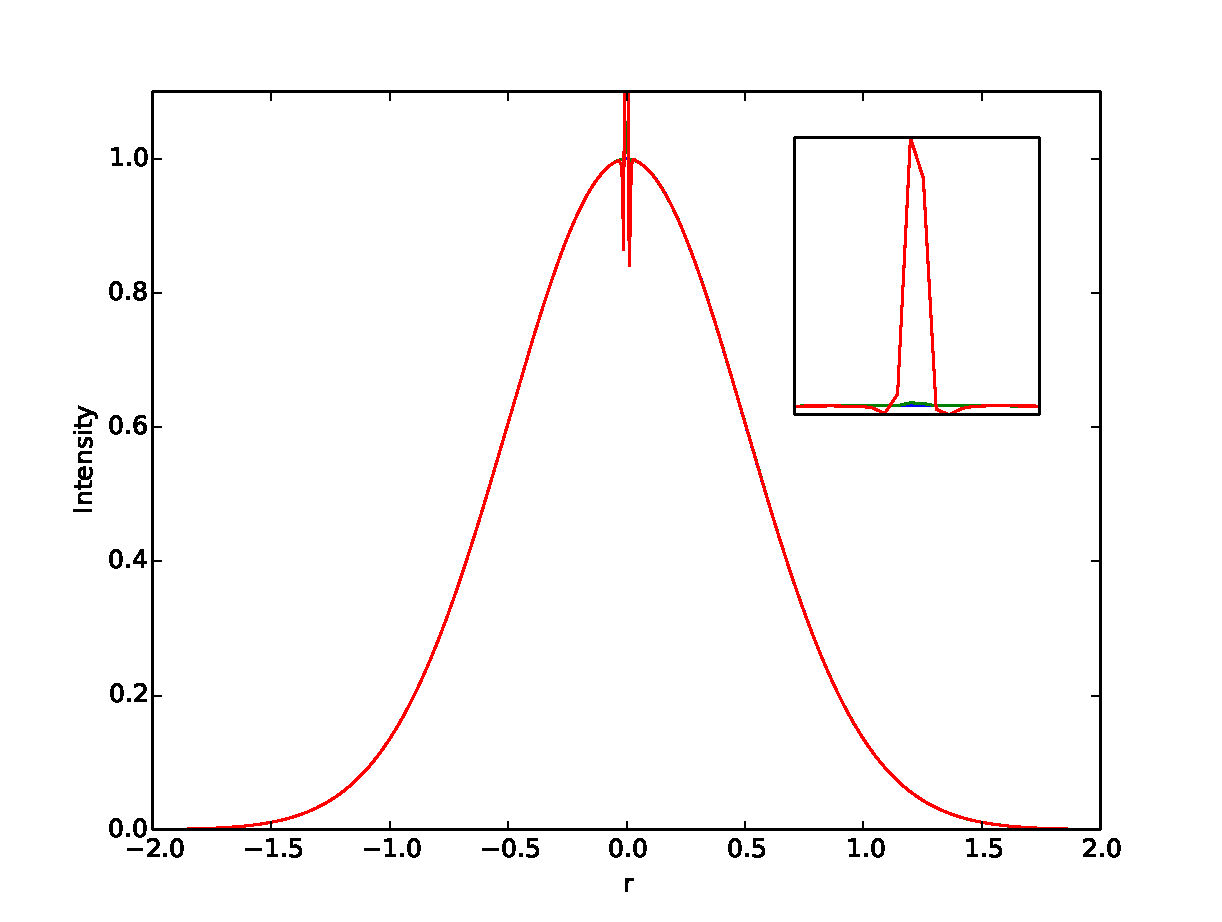
\includegraphics[width=0.45\columnwidth]{kerr_double}}
  \hfill
  \subbottom[Symmetric\label{fig:kerr-single}]{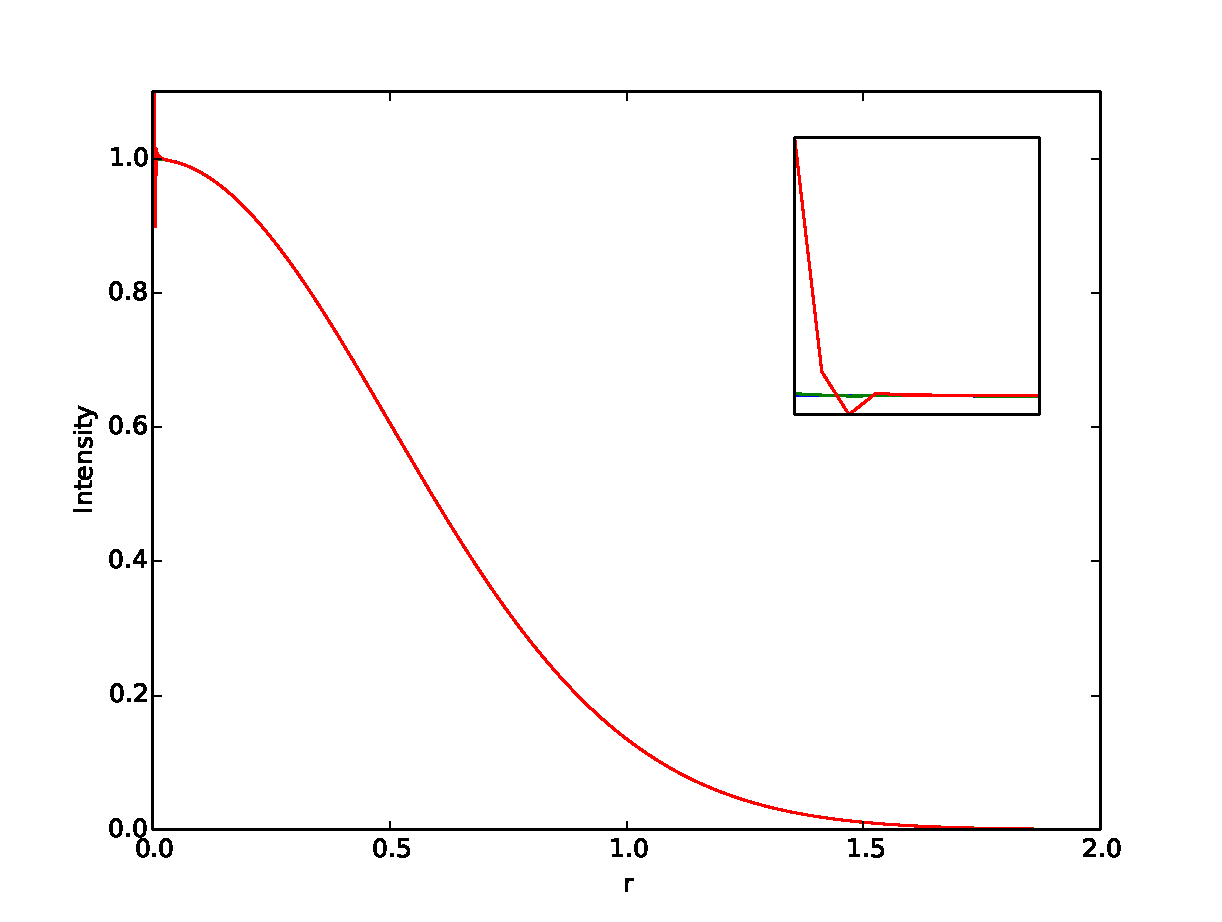
\includegraphics[width=0.45\columnwidth]{kerr_single}}
  \caption{The result of our nummerical simulation after propagating 10 steps. The insets shows the
    behavior around $r=0$.}
  \label{fig:kerr-num}
\end{figure}



%%% Local Variables: 
%%% mode: latex
%%% TeX-master: "nonlinear"
%%% End: 
